\documentclass[tikz,border=5pt]{standalone}
\usepackage{tikz}
\usetikzlibrary{arrows.meta}
\definecolor{nebula}{HTML}{6366F1}
\definecolor{spark}{HTML}{14B8A6}
\definecolor{sun}{HTML}{F59E0B}
\definecolor{ink}{HTML}{334155}
\begin{document}
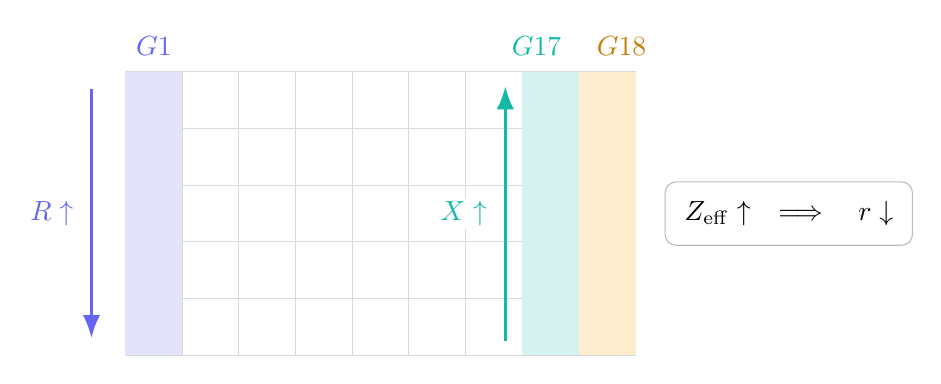
\begin{tikzpicture}[font=\sffamily,>=Latex,x=.72cm,y=.72cm]
  \foreach \x in {0,...,8}{\foreach \y in {0,...,4}{\draw[ink!20] (\x,\y) rectangle ++(1,1);}}
  \fill[nebula!18] (0,0) rectangle (1,5);
  \fill[spark!18] (7,0) rectangle (8,5);
  \fill[sun!20] (8,0) rectangle (9,5);
  \node[nebula] at (.5,5.45) {$G1$};
  \node[spark] at (7.25,5.45) {$G17$};
  \node[sun!80!black] at (8.75,5.45) {$G18$};
  \draw[->,very thick,nebula] (-.6,4.7)--(-.6,.3) node[midway,left=5pt,fill=white,inner sep=1pt] {$R\uparrow$};
  \draw[->,very thick,spark] (6.7,.25)--(6.7,4.75) node[midway,left=5pt,fill=white,inner sep=1pt] {$X\uparrow$};
  \node[draw=ink!35,rounded corners=4pt,fill=white,inner sep=7pt] at (11.7,2.5)
    {$Z_{\rm eff}\uparrow\quad\Longrightarrow\quad r\downarrow$};
\end{tikzpicture}
\end{document}
